\chapter{Individual texts}
\newpage
\textbf{Individual Page - Oscar Carlsson} \\\\
I've been sort of trying to act project manager, involving dividing equally amount of work on each group member and steering the project in the right direction. I've taught some basics in git in the beginning of the project and managed the repository with branches and such to make the the work easier for the others. All of us were new to Git so this has required some reading and supporting. \\\\
We wrote alot in teams and everyone has almost certainly edited every file some time during the project, but i will try to state which areas i've been most involved in. \\\\
We set up some scripts to process the documents into Matlab-friendly vectors. I contributed with a Snowball-stemmer, handling of arguments and pair-programmed TF-IDF etc. I were also involved in creating a nice way of generating feature vectors in .mat-format (such that all algorithms only needed to load the work space). Dealed with most areas of the datamanipulation.\\\\
All of us had prior knowledge of Machine Learning and we were able to re-use a lot of Matlab code. The original perceptron algorithm was at first written by me, but later on changed. I helped writing code to perform the classification tasks: In domain sentimental, Out of domain sentimental and Text categorization. Also spent some time to get nice plots of the data we received from the tests.\\\\
I started a lot of big and heavy tests on some of the computers at school. Started, collected data and made re-runs if there were any errors. E.g Training size-plot and Feature size-plot, both bigram and unigram.\\\\
In te final report i had the resposiblity for the parts related to Support Vector Machines, the paragraph about cross validation and wrote about our conclusions. But i, like the others, have been editing and writing in most of the chapters.\\\\
\newpage
\textbf{Individual Page - Oskar Ingemarsson} \\\\
I have been trying get involved in as much as possible in the project.
Very much have been done together in the group. This have been working
splendid and I think that this working style have benefited the project most
greatly. Since every one have touched almost everything the credit should go to
the group. I will however try to write something about what especially I have
done in the project.

I mainly been involved in processing the raw data from Amazon and work
concerning the implementation of perceptron. When it comes to the report I
mainly been writing the problem description, representing text, feature vectors
and KNN. Every body have been proofreading each others texts and re-regulated the
structure of the report under writing part of the project.

... and much more to write

%\section{Classifiers}

%\section{Report}
%Formost parts that are written by me in report is.
%\begin{itemize}
%\item Problem description
%\item Representing text
%\item K-Nearest Neighbour (KNN) algorithm
%\item Feature Vector / Text Representation
%\end{itemize}


\newpage
\section*{John Karlsson}
I have been largely involved in the following areas:
\begin{enumerate}
  \item Implementations
  \begin{enumerate}
    \item Naive Bayes
    \item SVM
    \item KNN
    \item Automation scripts and framework
    \begin{enumerate}
    	\item Data processing
    	\item Task procedures
    	\begin{enumerate}
    		\item Text categorization
    		\item Correlation analysis \& PCA
    	\end{enumerate}
    \end{enumerate}
  \end{enumerate}
  \item Report writing
  \begin{enumerate}
  \item Naive Bayes
  \item Results
  \end{enumerate}
\end{enumerate}
I have also spent a large part of my time participating in the collective and continuous planning, structuring and debugging of various parts of the project where needed. One important task has also been to manage, collect and discuss the test results.

\section*{Caroline Strandberg}
Much of the work we have done has been done together in the group and everyone have contributed with something to every part in both the implementation and the report. However, I will try to state which parts I have mainly been working with in project. 
\\\\
I have mainly been responsibly for the report and the Latex design of it. This has a involved making a structure for references and building a beginning structure for the report.
\\\\
When it comes to the implementation parts I have mainly been involved in writing the parser, used for the interpretation of the input string, together with Oskar. I have also been involved in writing the backend and blocks structure. 
\\\\
In the report I have mainly been writing the introduction chapter, i.e. Problem description and the Theory section involving The blocks world, SHRDLU, Grammatical Framework and A*. I have also been writing Programs and tools, Backend structure and Parser in the chapter Architecture. Furthermore, I have written the result, discussion, conclusion and future work. 
\\\\
I have also written the Reference list and format the documentation, given by the Haddock documentation for the code. But everyone in the group have read the whole report and been making small changes in every chapter.



\chapter{Plots}
\begin{figure}[H]
\centering
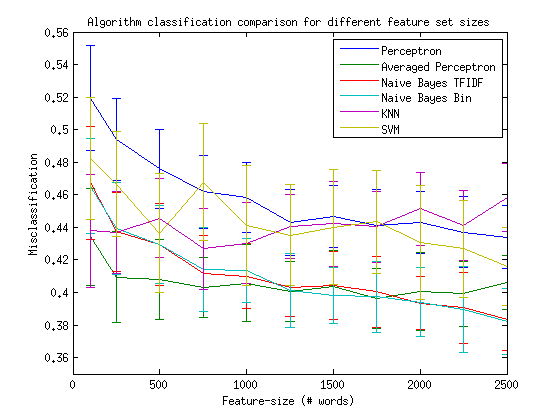
\includegraphics[scale = 1]{../Plottar/feature-size100-2500bigram.png}
\caption{In-domain classification using varying Bigram feature set sizes with 2$\sigma$ height error bars and comparing all algorithms.}
\end{figure} 

\begin{figure}[H]
\centering
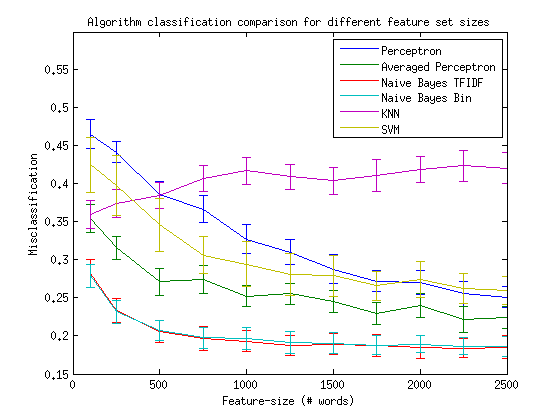
\includegraphics[scale = 1]{../Plottar/feature-size100-2500all.png}
\caption{In-domain sentiment analysis classification error (error bars of height $\sigma$) for the 6 algorithms on varying Unigram feature vector sizes}
\end{figure} 

\begin{figure}[H]
\centering
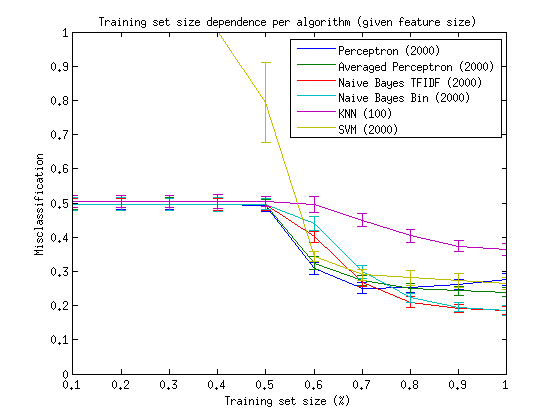
\includegraphics[scale = 1]{../Plottar/training_size_k_2000allknn_100.png}
\caption{Training set size dependence per algorithm}
\end{figure} 

\begin{figure}[H]
\centering
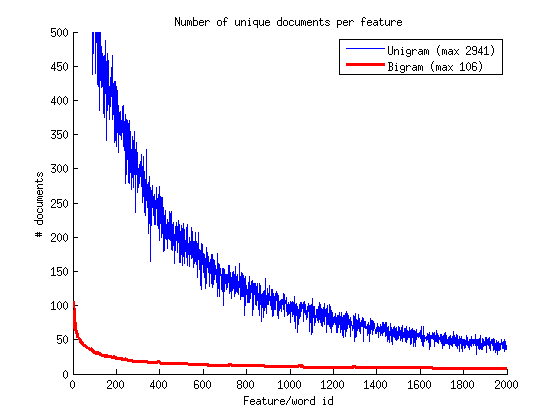
\includegraphics[scale = 1]{../Plottar/documents_per_feature.png}
\caption{Documents per feature. Bigram and Unigram}
\end{figure} 

\begin{figure}[H]
\centering
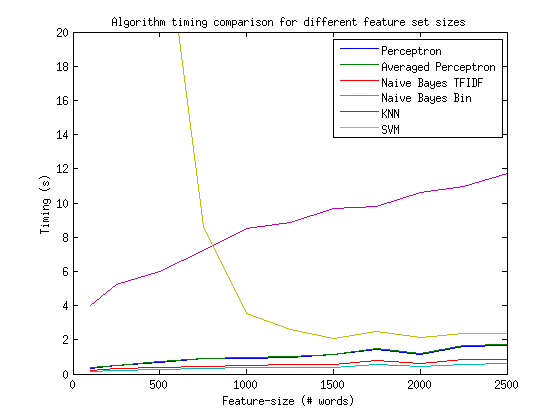
\includegraphics[scale = 1]{../Plottar/feature_size_TIMING.png}
\caption{Timing of different algorithms with different feature sizes}
\end{figure} 

\begin{figure}[H]
\centering
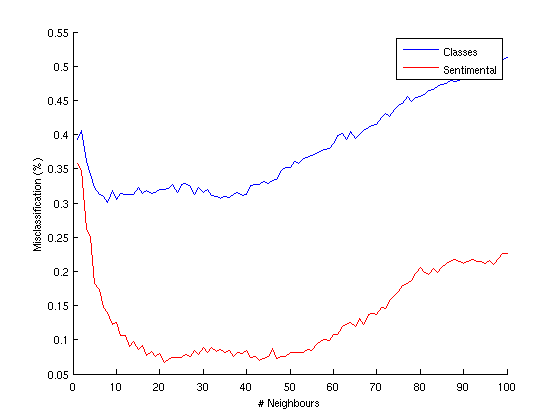
\includegraphics[scale = 1]{../Plottar/knn_2000words_testdata100_unigram.png}
\caption{Different K-values when running KNN on Classes and Sentimental-label}
\end{figure} 


\begin{sidewaysfigure}[H]
\centering
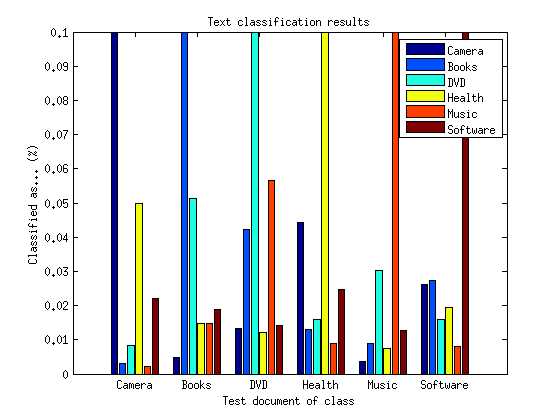
\includegraphics[scale = 0.47]{../Plottar/text_categorization.png}
\caption{Text categorization task}
\end{sidewaysfigure} 


\begin{sidewaysfigure}[H]
\centering
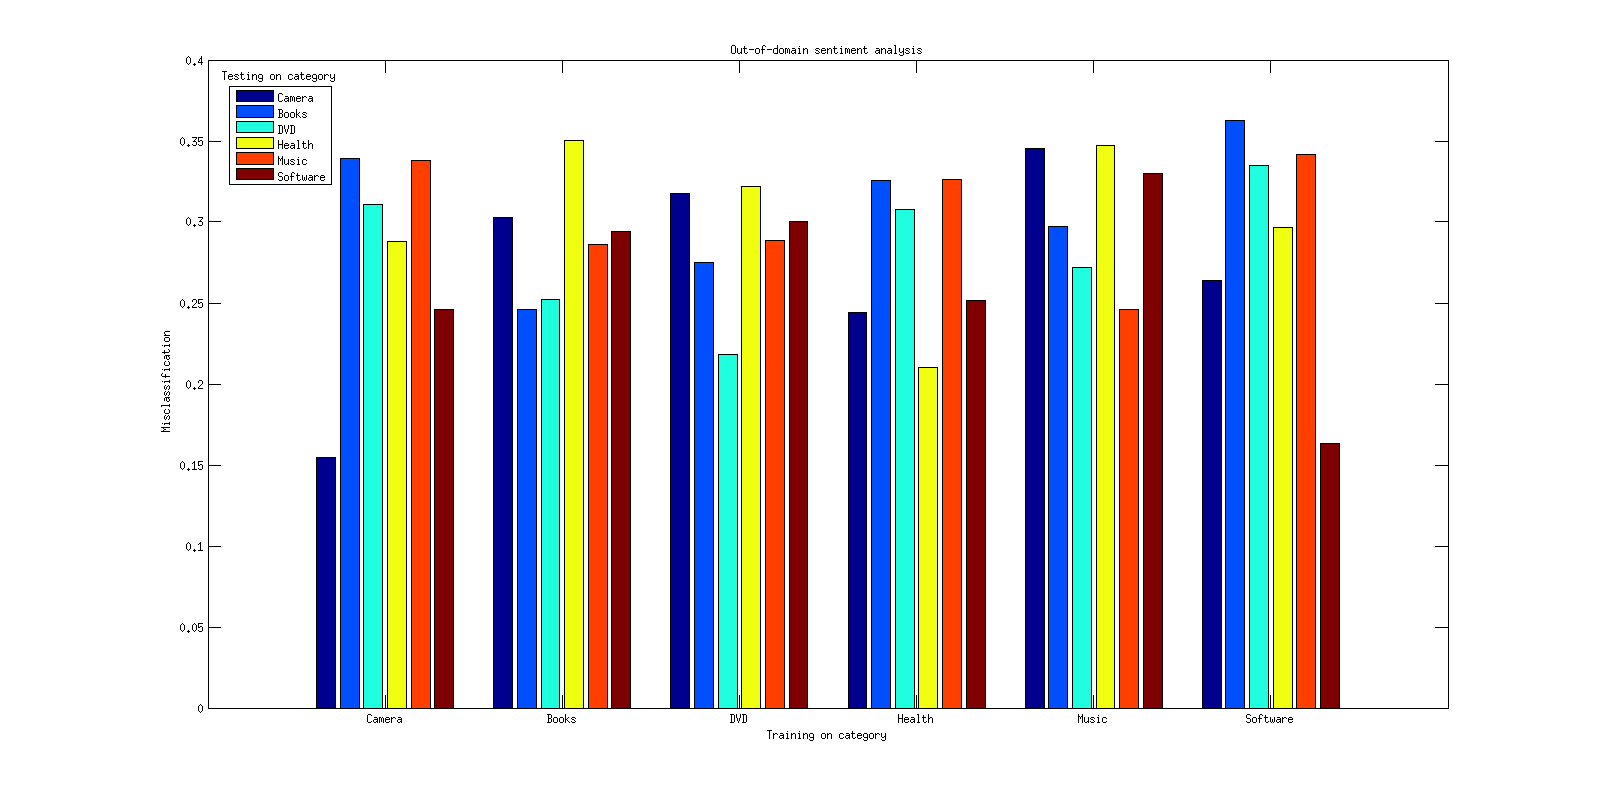
\includegraphics[scale = 0.47]{../Plottar/outofdomain.png}
\caption{Out of domain classification task}
\end{sidewaysfigure} 

\begin{figure}[H]
\centering
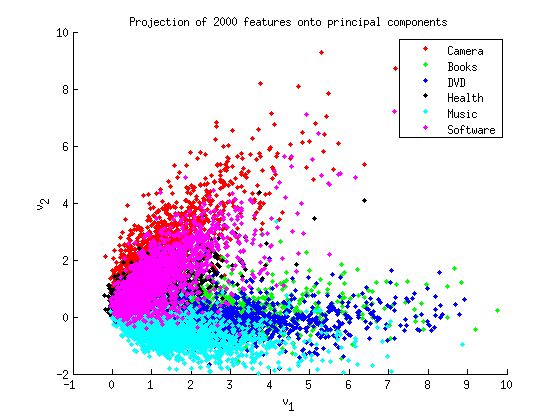
\includegraphics[scale = 1]{../Plottar/pca_all.png}
\caption{PCA on all categories}
\end{figure} 

\begin{figure}[H]
\centering
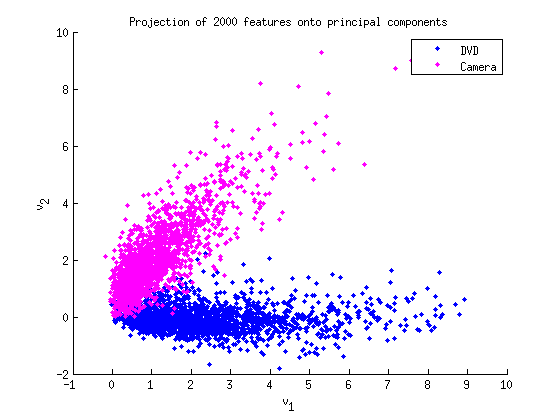
\includegraphics[scale = 1]{../Plottar/pca_nocorr.png}
\caption{PCA on DVD and camera with no correlation}
\end{figure} 

\begin{figure}[H]
\centering
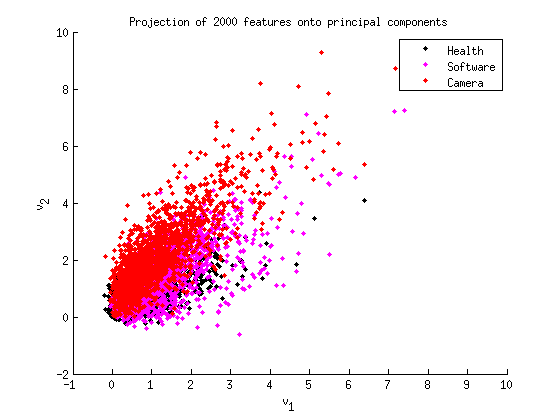
\includegraphics[scale = 1]{../Plottar/pca_largecorr.png}
\caption{PCA on health, software and camera. Represent a large correlation}
\end{figure} 

\begin{figure}[H]
\centering
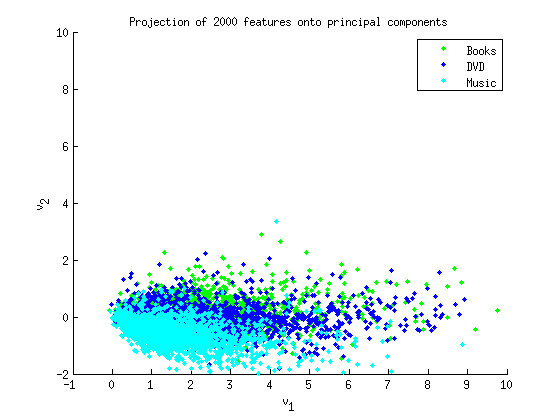
\includegraphics[scale = 1]{../Plottar/pca_somecorr.png}
\caption{PCA on Books, DVD and Music with some correlation}
\end{figure} 

\begin{figure}[H]
\centering
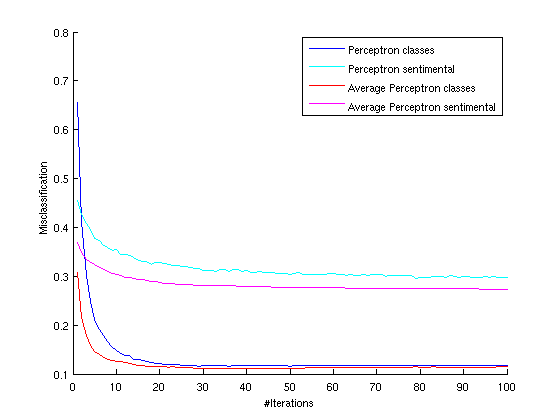
\includegraphics[scale = 1]{../Plottar/perceptron_2000words_unigram_10foldcv_classes-high_sentimental-low.png}
\caption{Different max iteration Perceptron}
\end{figure} 

\chapter{English stop words}
\input{appendix/english_word_stops.txt}

